\chapter{Introdução}
\label{c.introducao}

“Com o advento da realidade virtual e o avanço dos recursos computacionais, as representações interativas e imersivas do imaginário, bem como a reprodução do real, tornaram-se mais fáceis de serem obtidas.” \cite[p. ~9]{torilivro}

A realidade virtual (RV) vem ganhando espaço em diversos setores como jogos, indústria e educação. Na área de jogos, empresas como Playstation® e Oculus® oferecem um acervo de jogos para as suas respectivas plataformas. Ao procurar por jogos em RV na Google Play \cite{googleplay}, encontram-se algumas opções fornecidas por diversas empresas.

Na indústria, a RV pode ser utilizada para avaliar o design de um produto antes do mesmo ser produzido. A montadora \textit{The Ford Motor Company} é uma das empresas que utilizam a realidade virtual. Com esta tecnologia, é possível visualizar virtualmente tanto o exterior como o interior de um carro a ser produzido e avaliar aspectos de engenharia e design. “A realidade virtual pode ser mais efetiva do que desenvolver o design no mundo real. Só neste ano, designers e engenheiros verificaram mais de 135.000 detalhes em 193 protótipos virtuais de veículos” \cite[tradução nossa]{ford}. 

Já na área da educação, a realidade virtual pode ser aplicada por meio de jogos educativos e aulas imersivas. Imagine utilizar a RV em uma aula de história para simular um acontecimento histórico, ou ter a sensação de estar no espaço enquanto assiste uma aula de astronomia. Pesquisas como \cite{youngblut} e \cite{carvalho} mostram como a realidade virtual pode ser incorporada na escola.

Para se obter uma experiência em realidade virtual, são necessários capacetes de visualização ou óculos de RV, um \textit{display} por onde a aplicação irá rodar, um dispositivo de interação e a aplicação em RV. 

Atualmente existem vários modelos de óculos de RV com suporte à realidade virtual, tais como: Oculus Rift da Oculus® com preço estimado em R\$ 4.620,90 e Samsung Gear VR da Samsung® (R\$ 799,00). No entanto, o Google Cardboard da Google® é o que possui preço mais acessível em torno de R\$ 21,97 possuindo atualmente duas versões, cada uma com um meio de interação próprio. Em novembro 2016, a Google® lançou um novo visualizador denominado Daydream (Figura ~\ref{f.daydream}). Este visualizador acompanha um controle com comunicação \textit{Bluetooth} e o capacete de visualização feito com tecido para garantir maior conforto, além de um suporte para fixação do visualizador à cabeça do usuário. Os \textit{smartphones} compatíveis com o Daydream são os que possuem Android 7.0 (Nougat) ou superior. Outras versões do Android, apesar de serem compatíveis com aplicações em RV, não oferecem suporte para o controle do Daydream.

\begin{figure}[ht]
	\caption{\small Daydream}
	\centering
	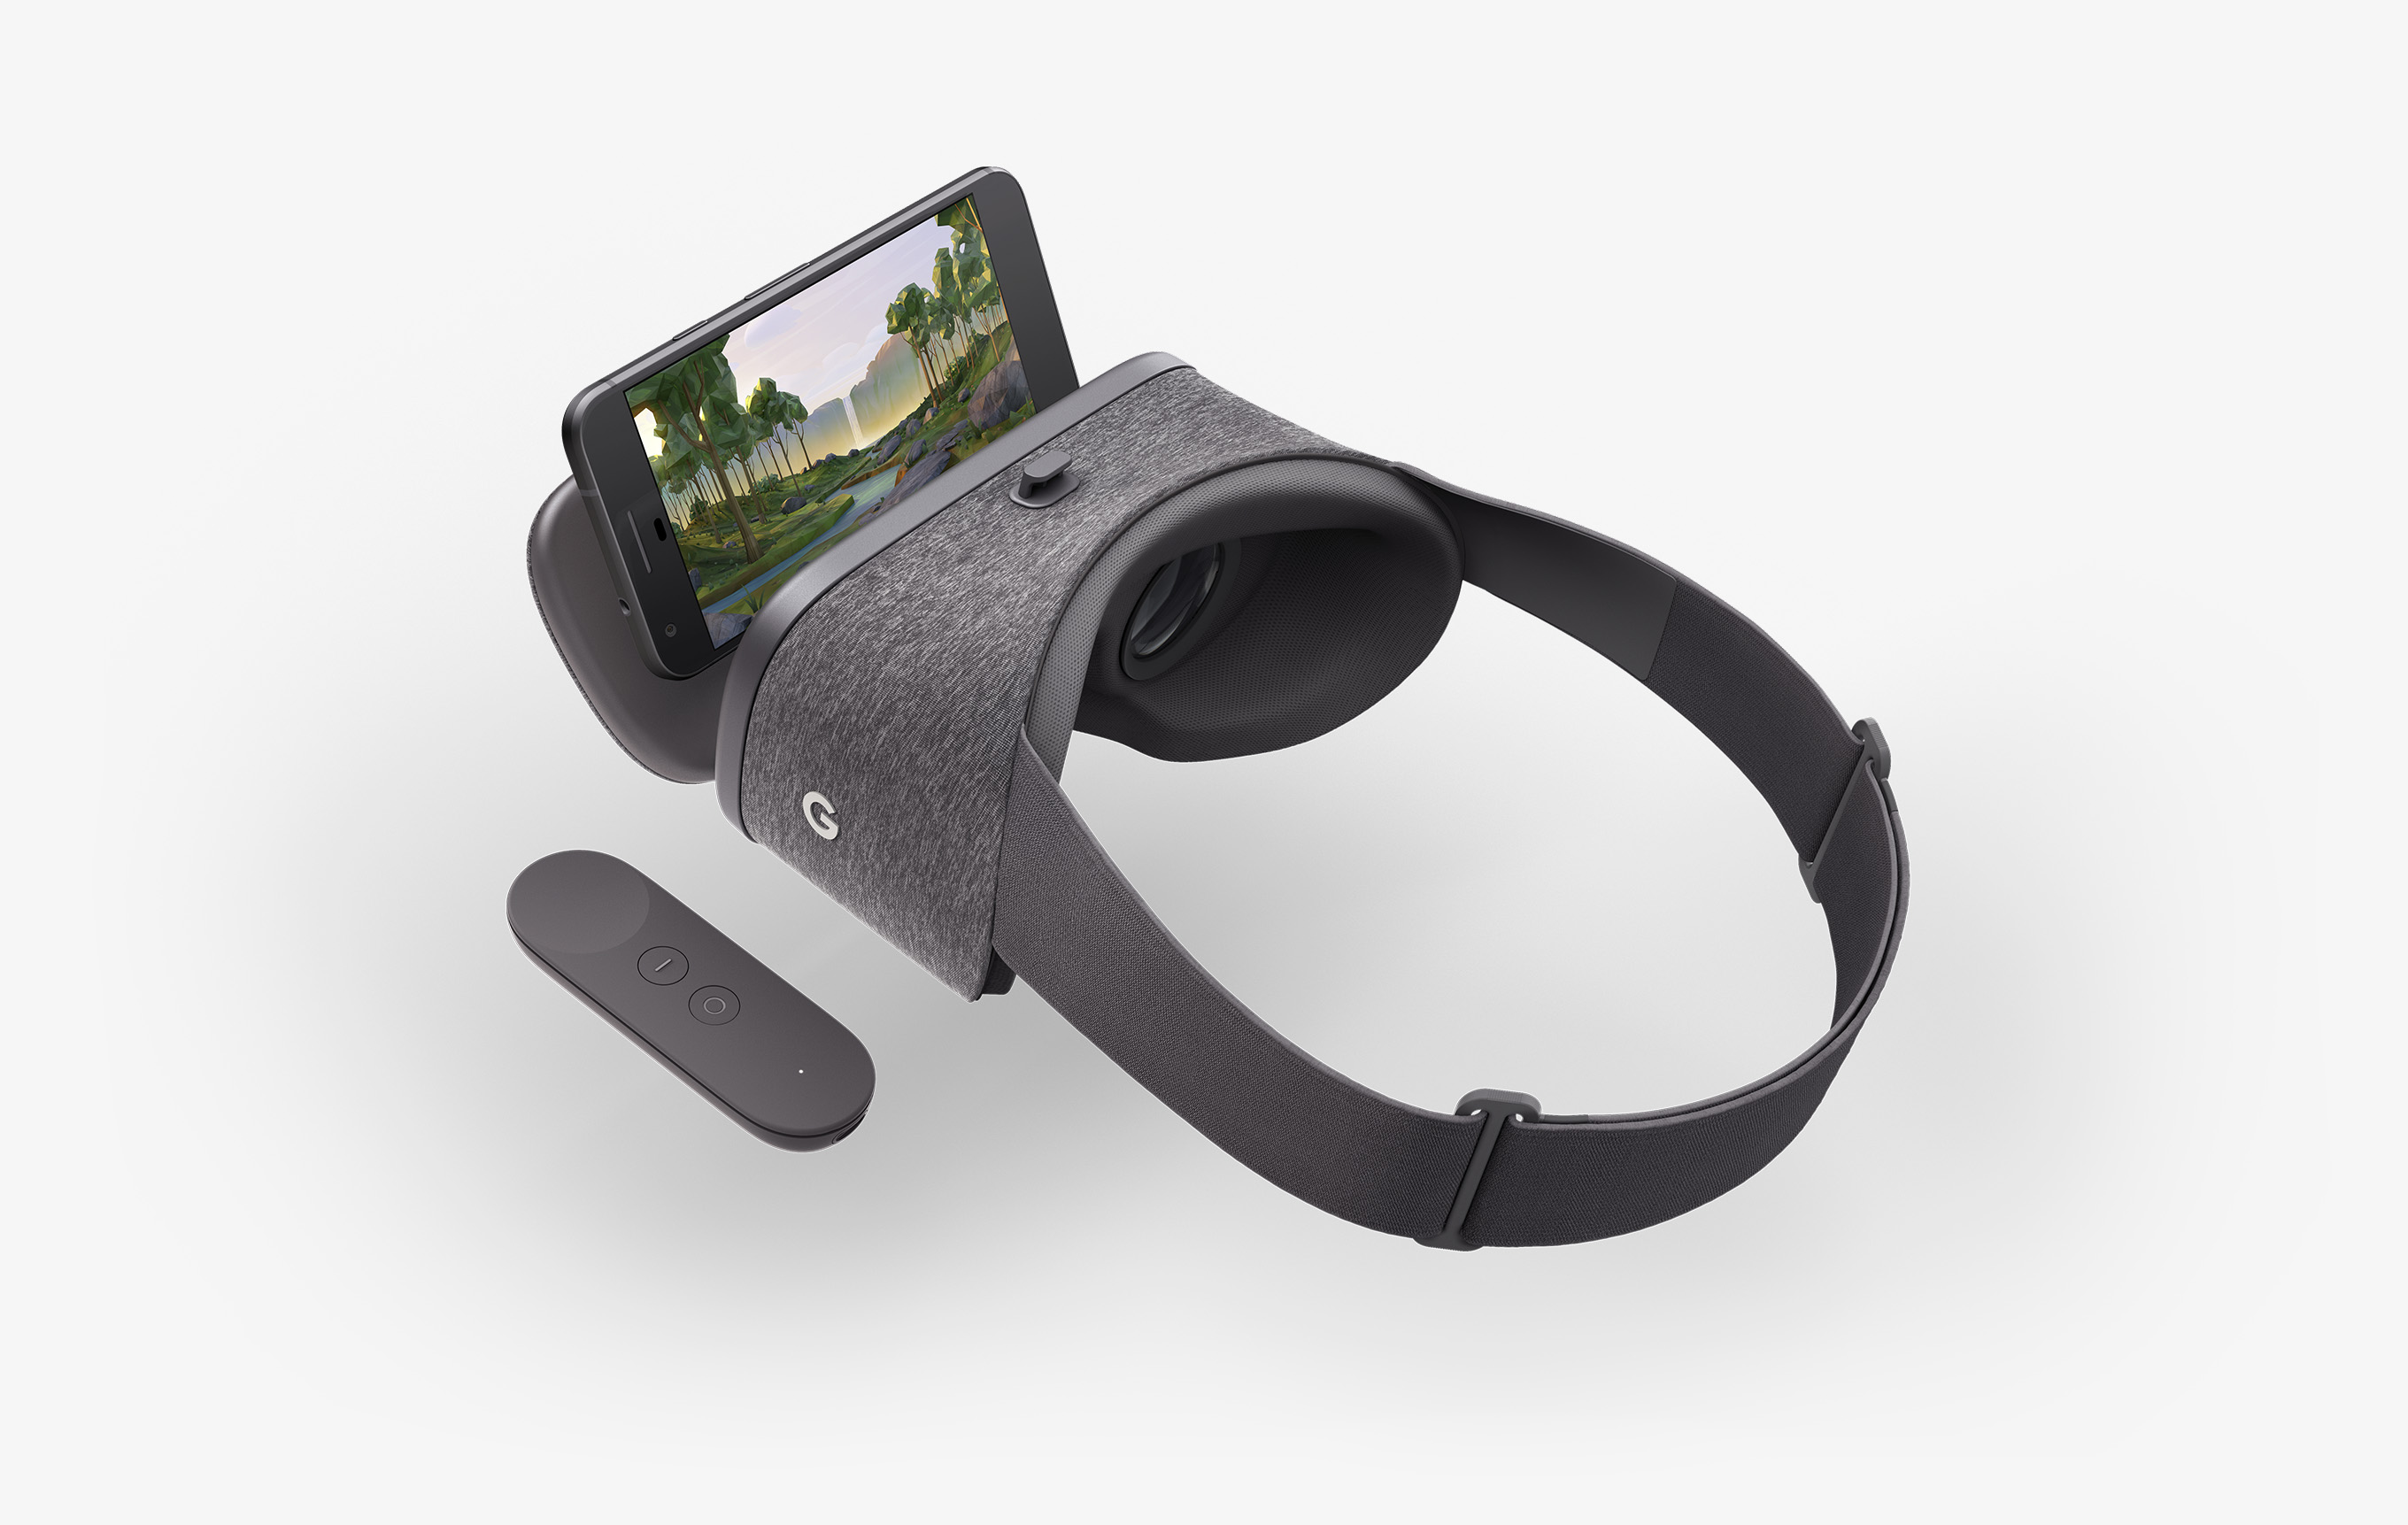
\includegraphics[scale=0.15]{Imagens/daydream.jpg}
	\label{f.daydream}
	\legend{\small Fonte: \cite{daydream}}
\end{figure}

As aplicações em RV podem ser desenvolvidas tanto para computadores como para dispositivos móveis. A principal diferença entre as duas plataformas é a capacidade de processamento e memória, que são inferiores nos dispositivos móveis. Para as aplicações \textit{desktop} utiliza-se óculos de RV como o Oculus Rift para executar a aplicação. Já nas aplicações para dispositivos móveis, é necessário um visualizador como o Google Cardboard por onde o \textit{smartphone} será encaixado.

Em todos os casos, uma aplicação em realidade virtual deve permitir algum tipo de interação. Para isso, com o visualizador posicionado na cabeça do usuário, é possível utilizar a movimentação da cabeça e um controle externo como luvas, mouse 3D, \textit{joystick}, entre outros. A grande dificuldade é encontrar uma forma de interação que seja viável e que garanta usabilidade e experiência satisfatórias aos usuários. “A necessidade de se fazer uso de aparatos tecnológicos para a interação do usuário com o ambiente virtual provoca restrições, tanto pelo aspecto econômico e tecnológico, quanto pelo desconforto, mas permite ao usuário fazer coisas que antes eram impossíveis ou inviáveis. ” \cite[p. ~3]{torilivro}

Este projeto utiliza óculos de RV e um dispositivo móvel para criar uma aplicação que explora os conceitos da realidade virtual visando explorar diferentes formas de interação utilizando controles externos.

\section{Problema}
\label{s.problema}

Apesar da quantidade de aplicações desenvolvidas utilizando RV para dispositivos móveis estar em crescimento, ela é pequena em comparação com aplicações para \textit{smartphones} sem a tecnologia de RV. Além disso, os estudos de formas de interação com aplicações em RV que possam propiciar conforto, eficácia e conectividade adequada com \textit{smartphones} são atuais. 

O Google Cardboard versão 1 propõe apenas duas formas de interação com o usuário: Movimentação da cabeça e um par de ímãs que, quando utilizados representam um toque na tela, seu funcionamento é ilustrado na Figura ~\ref{f.cardboard1}. Já a versão 2 não possui ímãs e utiliza o toque na tela como forma de interação como é ilustrado nas Figuras ~\ref{f.botaocardboard1} e ~\ref{f.botaocardboard2}. Atualmente, o suporte para a interação via ímã está sendo descontinuado e, por isso, as análises foram feitas utilizando o Google Cardboard versão 2.

\begin{figure}[H]
	\caption{\small Funcionamento do ímã}
	\centering
	\includegraphics[scale=0.7]{Imagens/cardboard.png}
	\label{f.cardboard1}
	\legend{\small Fonte: Elaborada pelo autor.}
\end{figure}

\begin{figure}[H]
	
	\begin{minipage}{.5\textwidth}{
			\centering
			\captionof{figure}{\small Botão pressionado}
			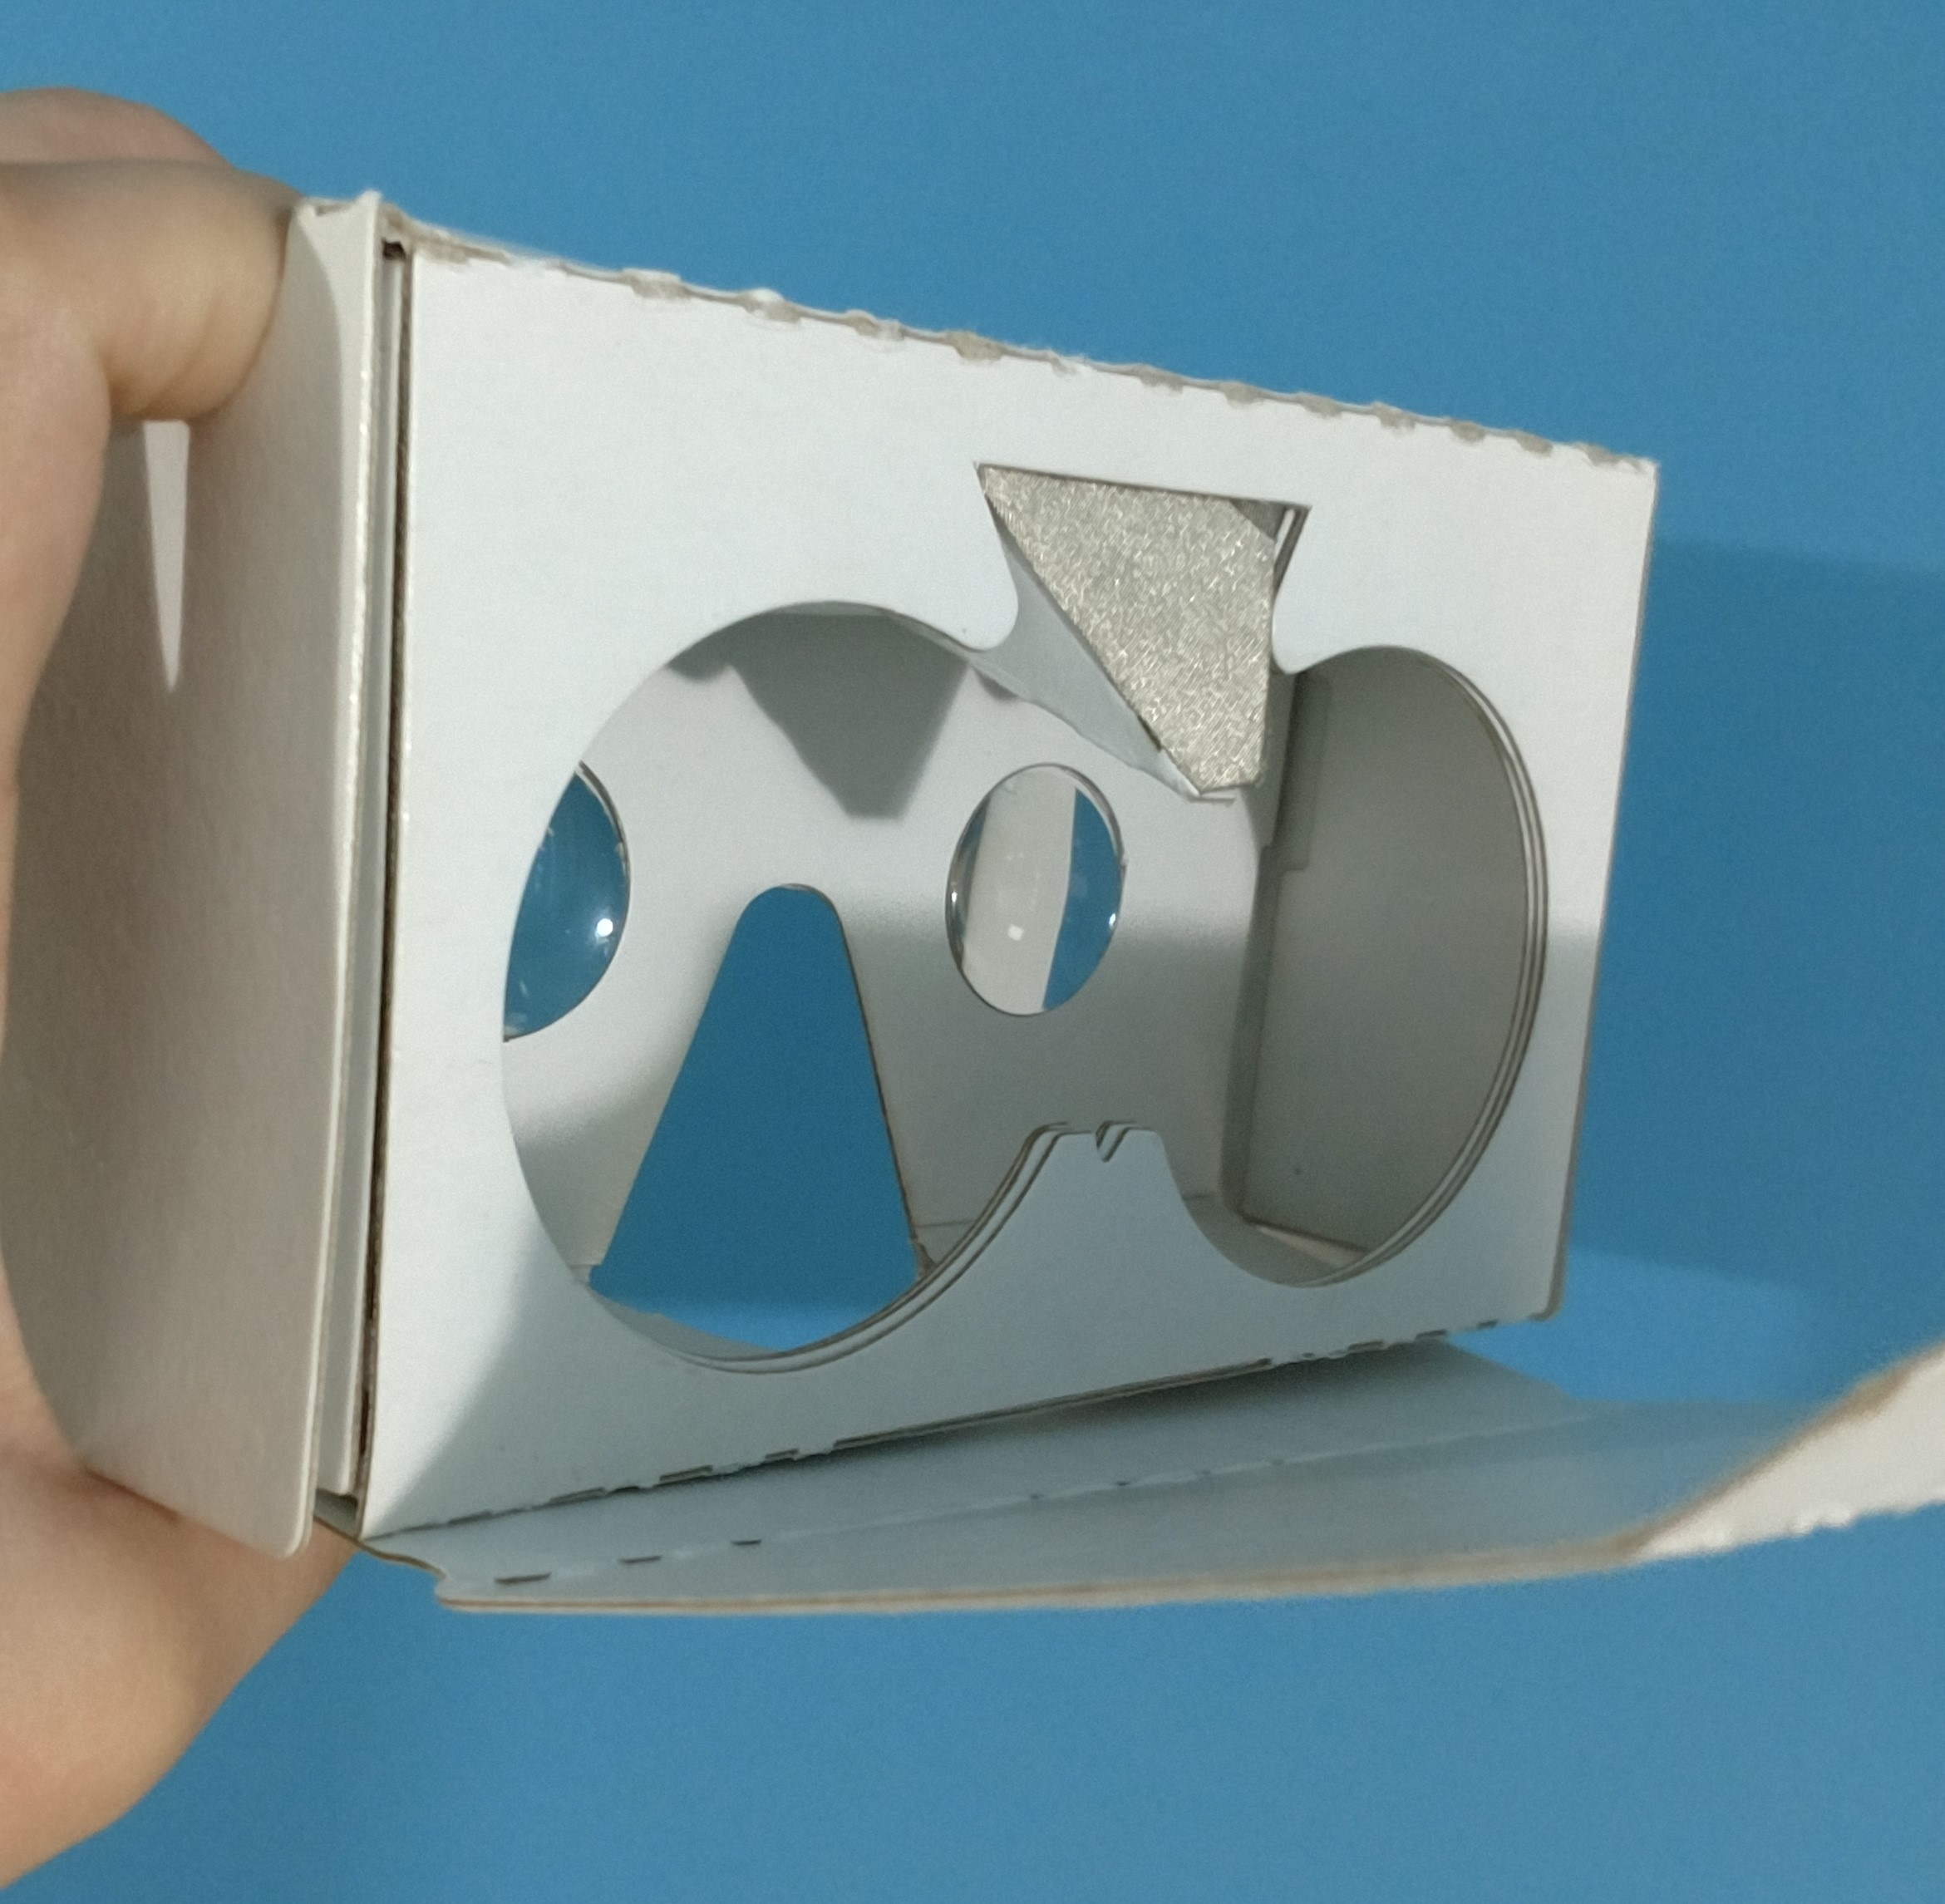
\includegraphics[height=5cm]{Imagens/botaocardboard1.jpg}		
			\label{f.botaocardboard1}
			\legend{\small Fonte: Elaborada pelo autor.}	
		}
	\end{minipage}
	\begin{minipage}{.5\textwidth}{
			\centering
			\captionof{figure}{\small Liberação do botão (toque na tela)}
			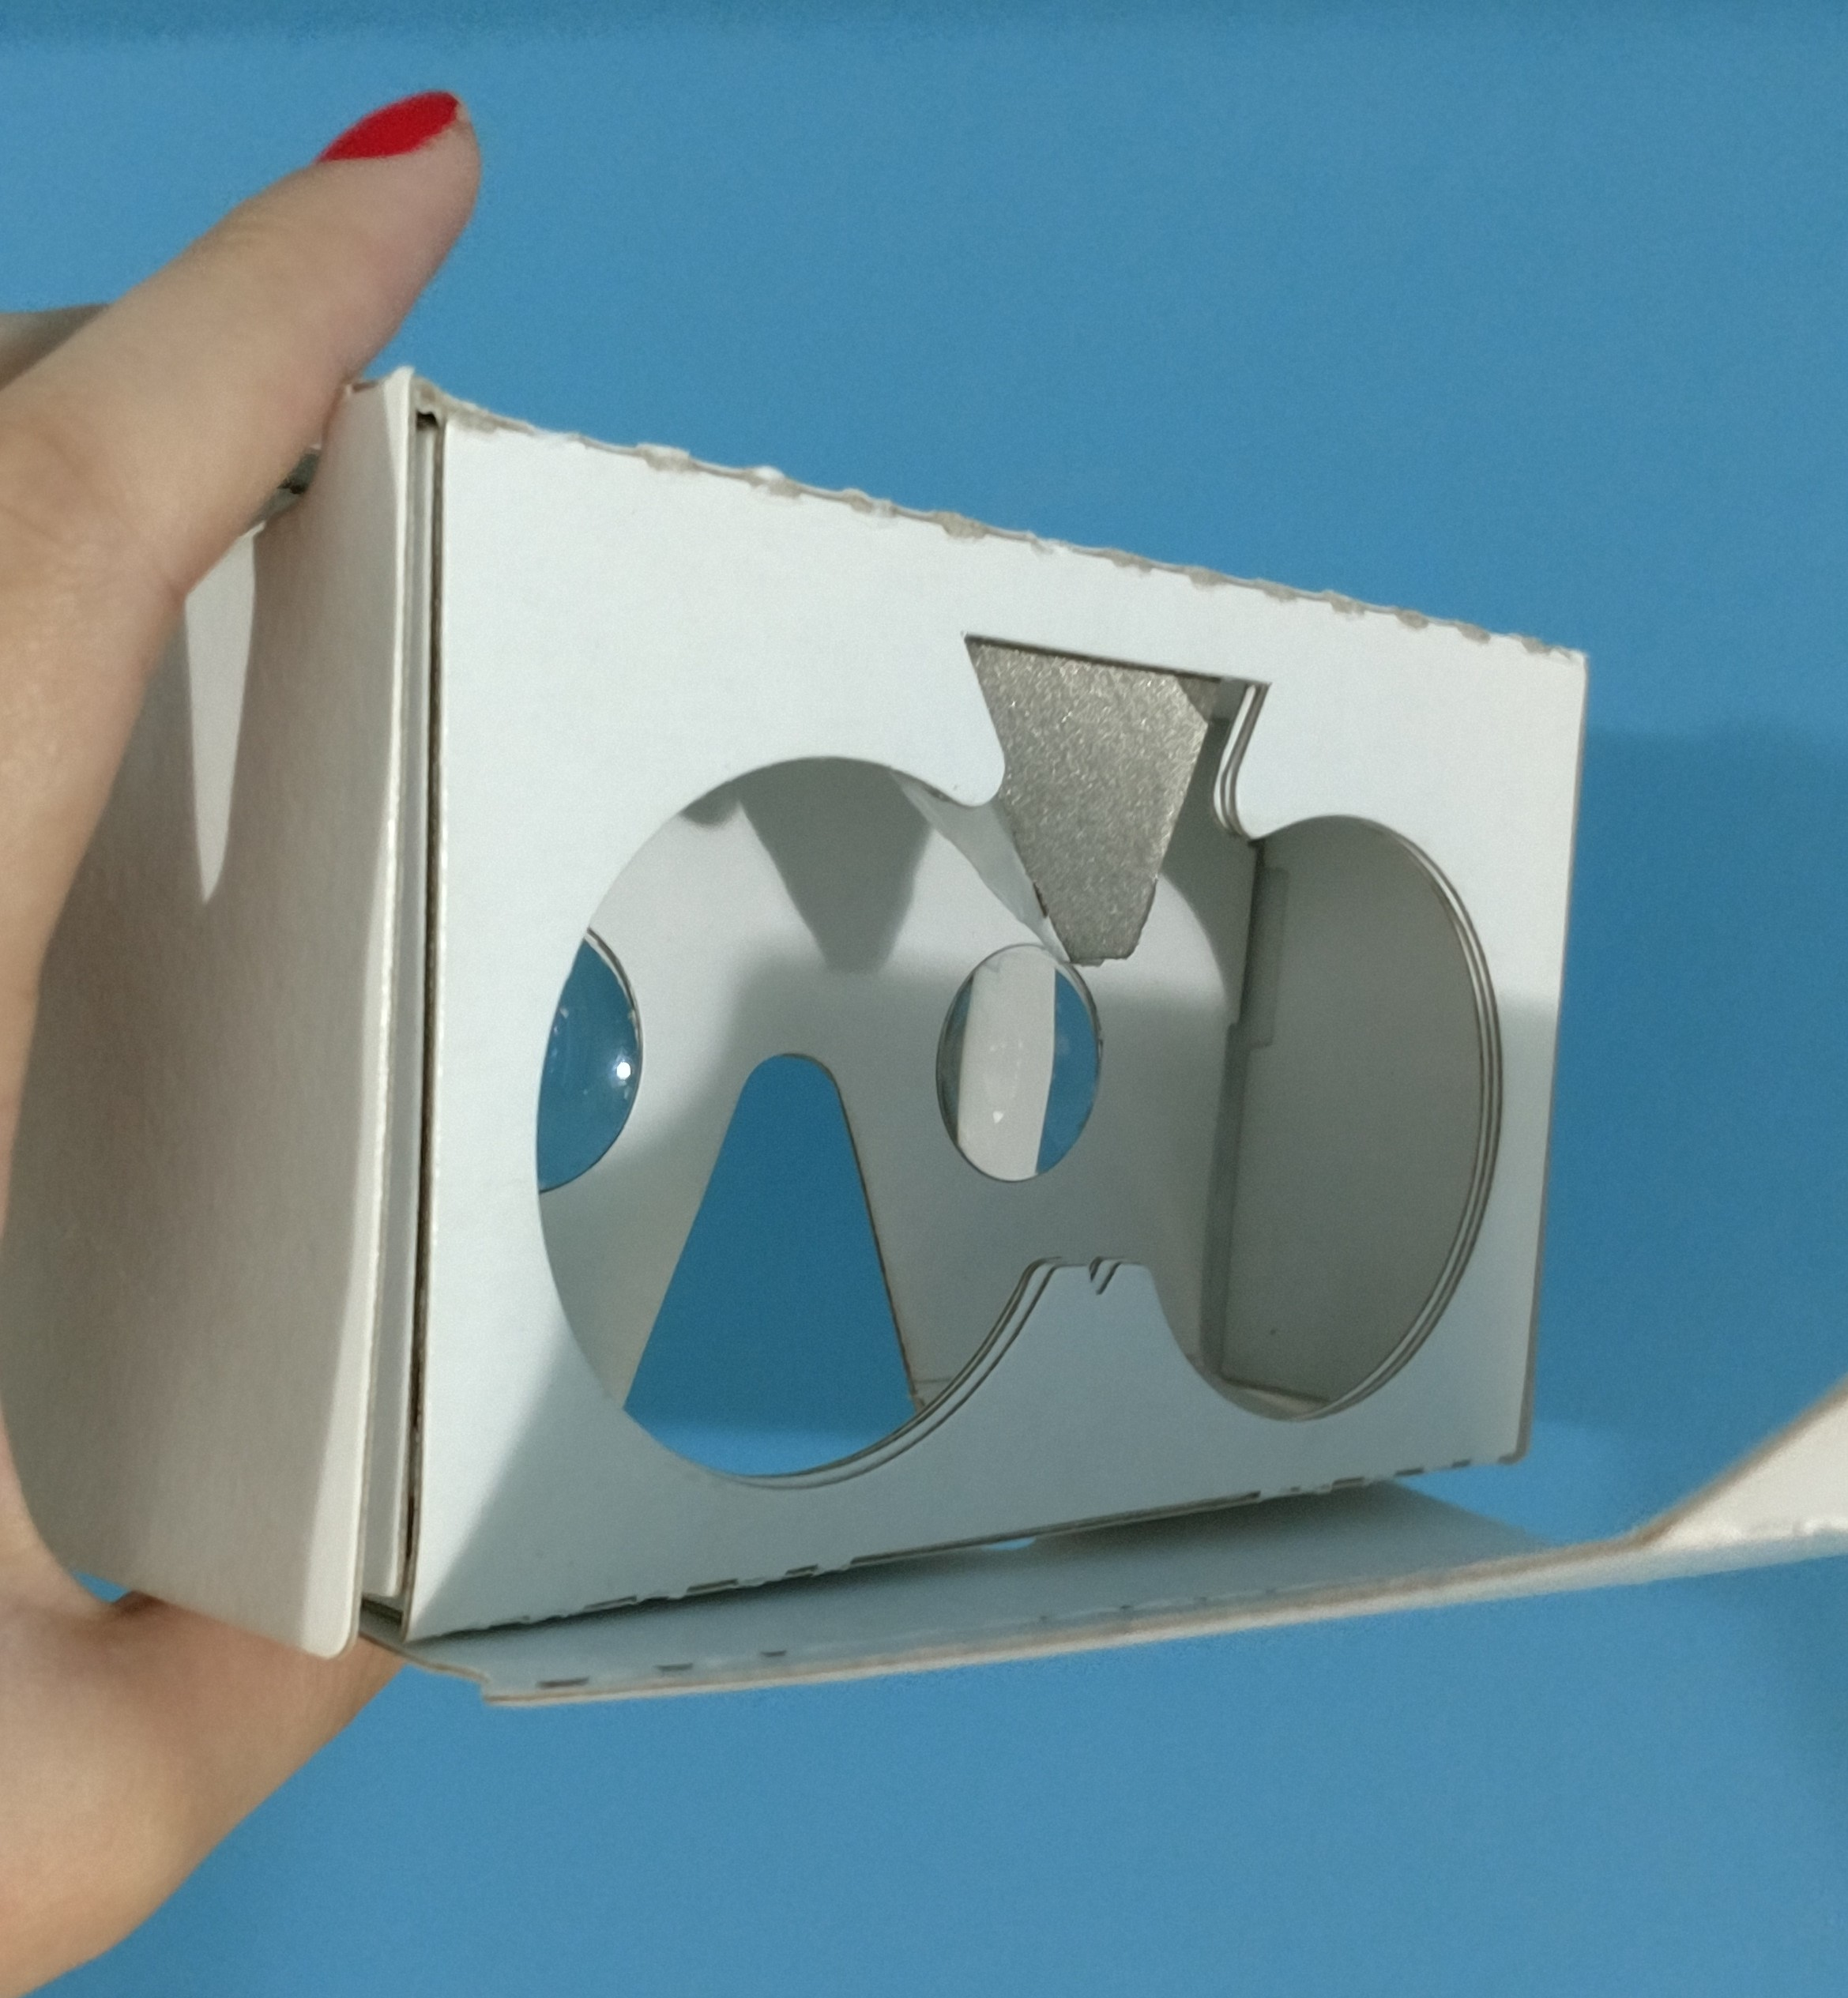
\includegraphics[height=5cm]{Imagens/botaocardboard2.jpg}		
			\label{f.botaocardboard2}	
			\legend{\small Fonte: Elaborada pelo autor.}
		}
	\end{minipage}
\end{figure}

Contar apenas com duas formas de entrada de dados, limita as opções de interação do usuário com a aplicação. A empresa Oculus®, vende seus óculos de RV juntamente com um controle de vídeo game, o que garante maior flexibilidade na criação de aplicações em RV. No entanto, a diferença de preço entre o Google Cardboard e o Oculus Rift é significativa, isto é,  o primeiro custa aproximadamente duzentas vezes o preço do segundo.

Encontrar formas de interação ótimas para um determinado ambiente é um problema muito estudado na área de Interação Humano-Computador pois, com os avanços tecnológicos, surgem novas possibilidades de interação. É o caso da realidade virtual, onde o usuário utiliza o próprio corpo como forma de entrada de dados. Também é possível utilizar um controle externo para ações adicionais, no entanto, a escolha deste controle precisa ser estudada.

\begin{citacao}
A grande maioria dos usuários não consegue dominar todas as funcionalidades de um sistema antes que mais funções sejam adicionadas, isso acontece porque com a evolução tecnológica caminhando a passos largos, as novas possibilidades saltam aos olhos dos fabricantes de hardware e desenvolvedores de software, celulares equipados com GPS, câmeras digitais com reconhecimento facial, telas sensíveis ao toque, jogadores controlando jogos apenas movimentando o próprio corpo, interação com objetos virtuais através da realidade aumentada, interação ativa do telespectador com a televisão. Todas essas tecnologias desafiam os fabricantes a criar interfaces que possibilitem o acesso a essas novidades sem perder a objetividade e a clareza. \cite{oliveira}
\end{citacao}

\section{Justificativa}
\label{s.justificativa}

A realidade virtual é um tema em expansão, objeto de pesquisa de grandes empresas como o Facebook® e a Google®. Logo, investigar formas de utilização desta tecnologia em dispositivos móveis como \textit{smartphones} é contribuir com conhecimento para a área bem como auxiliar o trabalho de desenvolvedores. 

É interessante apresentar formas diferentes de interação com aplicações em RV e, ao mesmo tempo, obter uma experiência em realidade virtual acessível. O sistema operacional Android oferece bibliotecas que ajudam no tratamento de diversos meios de entradas como \textit{Bluetooth} e via cabo. Além disso, os \textit{smartphones} atuais possuem sensores como acelerômetro e giroscópio que são utilizados para o desenvolvimento de aplicações em RV. Com o auxílio dos recursos mencionados, é possível realizar uma comparação entre diversos tipos de controles físicos, a fim de escolher o mais apropriado para ser utilizado em uma aplicação em RV. 

Por fim, o projeto pode ser realizado com materiais de baixo custo e de fácil acesso, podendo ser encontrados softwares completamente gratuitos.

\section{Objetivos}
\label{s.objetivos}

\subsection{Objetivo Geral}
\label{s.geral}
Explorar formas de interação do usuário em aplicação de RV executada em dispositivos móveis por intermédio de um controle externo.

\subsection{Objetivos Específicos}
\label{s.especifico}
- Identificar os elementos necessários para a criação de uma aplicação em RV.

- Definir as principais restrições na escolha e ferramentas de RV para construção da aplicação.

- Identificar dispositivos físicos como forma de controle na interação entre o usuário e a aplicação RV.

- Realizar a análise dos controles físicos.
